\chapter{Architettura di sistema}

Affinché l'utente sia agevolato nello sviluppo di un firmware, egli deve sfruttare al meglio l'interoperabilità dei componenti e le potenzialità dell'intero sistema di sviluppo.

Risulta quindi necessaria una visione di insieme dell'intero sistema invece che una valutazione locale dei singoli componenti oltre che a una valutazione della compatibilità inter-componente affinché la loro interazione permetta allo sviluppatore di operare con facilità.

\begin{figure}[t]
    \centering
    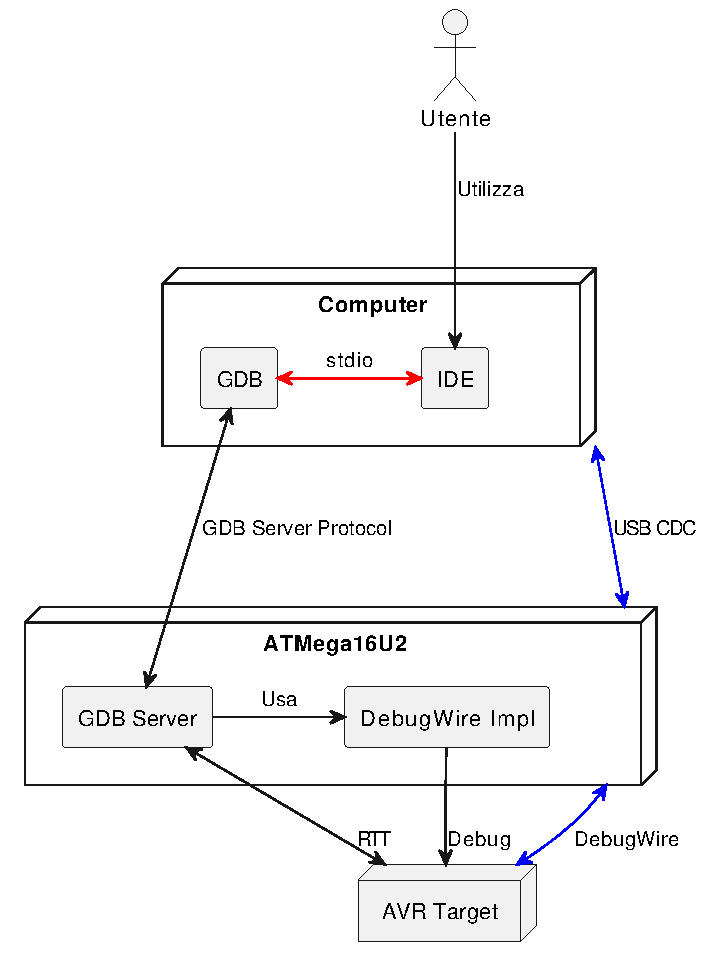
\includegraphics[width=.7\textwidth]{sys-arch.pdf}
    \caption[]{Diagramma dei componenti del sistema di assistenza alla programmazione e debugging}\label{fig:sys-arch}
\end{figure}

Come osservabile dalla \cref{fig:sys-arch}, il sistema sviluppato si basa su tre livelli fisici collegati a cascata da conessioni fisiche (indicate in blu nella figura), in modo tale da adattare le azioni ad alto livello scelte dall'utente ai comandi di basso livello che permettono di interagire con il controllore \textit{target}, interagendo tra di essi mediante l'ausilio di connessioni logiche di protocolli incapsulati nelle connessioni fisiche. 

Il primo livello, ovvero il livello di interfaccia con lo sviluppatore, consiste nel software utilizzato per lo sviluppo del firmware contenente tutti gli strumenti di supporto alla programmazione. Questi software, anche noti come IDE\footnote{Integrated Development Environment}, hanno il compito di accorpare svariate funzionalità mediante integrazione di software esterni allo scopo di favorire lo sviluppo fornendo un ambiente unico e integrato allo sviluppatore, dal quale effettuare tutte le operazioni quali sviluppo, compilazione, debugging e upload.

Enfasi particolare viene posta sull'integrazione da parte dell'IDE del supporto al software GDB, il quale svolge il compito di processo \textit{debugger}, ovvero il processo responsabile della gestione delle richieste al server di debug per controllare il comportamento e il flusso di esecuzione di un processo \textit{target} nominato ``processo \textit{debuggee}''.

Il \textit{debugging} è una delle pratiche ormai fondamentali della programmazione che permette una comprensione agevolata del flusso di esecuzione del codice e permette di ispezionarne i vari stati.

In particolare esso garantisce la possibilità di analizzare uno stato intermedio tramite l'esecuzione del codice in modo interattivo, consentendo allo sviluppatore di condurre ``un'indagine'' relativa a un funzionamento inatteso del firmware. Metaforicamente possiamo affermare che il \textit{debugging} sia paragonabile ad un'indagine condotta dallo sviluppatore dove egli stesso è il colpevole.

È necessario porre un'ulteriore enfasi sull'aggettivo ``interattivo'': la differenza tra \textit{debugging} e \textit{logging} sta proprio nel fatto che il secondo consiste solamente nella stampa, su un terminale o file, di una serie di messaggi statici e predefiniti al fine di tracciare gli eventi per un'analisi futura di un evento inaspettato. Ciò non permette quindi di effettuare decisioni in funzione dei risultati parziali ottenuti nella procedura di \textit{debugging} a meno di riprogrammare il dispositivo --- inficiando così la longevità delle memorie e comportando un uso inefficiente del tempo --- e ricapitolare l'esecuzione del codice.

Risulta quindi di grande importanza poter accedere a uno (o più) software per il debugging in modo che esso possa essere efficiente.
Uno dei software più utilizzati per il debugging del codice compilato, è Gnu GDB\cite{site:gdb}.

\section{Gnu Debugger}\label{sec:gdb}

Il software GDB è un debugger multi-architettura\cite{site:gdb} utilizzato per l'ispezione degli stati di esecuzione dei software compilati.
In particolare esso presenta un'architettura multipla di funzionamento in funzione della localizzazione del processo da ispezionare.

Generalmente il processo da analizzare è direttamente localizzato sulla stessa macchina nella quale il processo GDB viene istanziato. In questo caso è sufficiente utilizzare delle chiamate di sistema (\textit{syscall}) in grado di bloccare l'esecuzione del processo e accedere alla memoria a lui dedicata.
Sarà dunque possibile modificare il contenuto della porzione di memoria in cui è caricato l'eseguibile in modo da sostituire l'istruzione incriminata con un'istruzione di ``\textit{break}''. Questa istruzione causerà, al momento della sua esecuzione, un'eccezione a livello hardware la quale verrà gestita dal kernel e notificherà il processo \textit{debugger} che il processo \textit{debuggee} ha raggiunto un \textit{breakpoint}.

Purtroppo non sempre il processo \textit{debuggee} è in esecuzione sullo stesso processore in cui si trova il processo GDB client. Questo comporta la necessità di scindere in due componenti il programma utilizzato per effettuare il \textit{debug} adottando un'architettura client-server per consentire la dislocazione del server permettendo a quest'ultimo di interagire con il processo \textit{debuggee}.

\subsection{Debugging di dispositivi embedded}

Quanto enunciato precedentemente si avvera nel debugging di dispositivi embedded. 

Possiamo vedere il firmware in esecuzione sul microcontrollore come un processo dislocato su un processore remoto con una diversa architettura.

La problematica relativa alla diversa architettura dei processori non costituisce motivo di preoccupazione in quanto ormai la maggior parte degli \textit{instruction set} è stata inclusa nella distribuzione di GDB multi-architettura\cite{site:gdb}.
La vera problematica si ha con la scarsa connettività dell'integrato, la quale richiede un protocollo e un componente di adattamento \textit{ad-hoc}.
L'architettura client-server permette quindi di implementare tale adattatore su un dispositivo esterno connesso con il \textit{target} avente possibilità di implementare il protocollo di debug permettendo così di adattare l'interfaccia a tutti i dispositivi in grado di eseguire GDB.\@ 

Possiamo vedere come la concezione di separazione tra applicativo di controllo e interazione ed esecutore dei comandi di debug può essere implementata dalla \cref{fig:gdb-server-tunnels}.

\begin{figure}
    \centering
    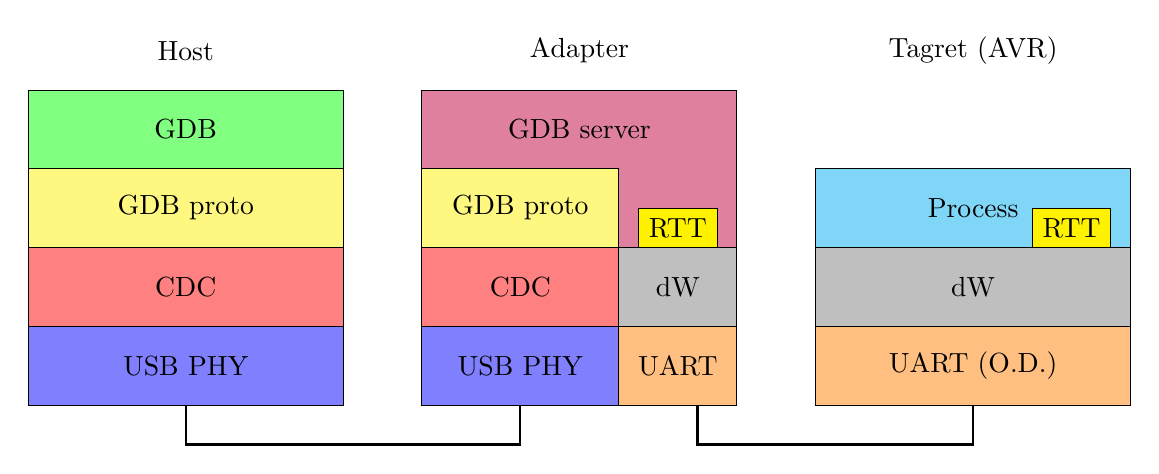
\begin{tikzpicture}
        \draw[fill=green!50] (0,3) rectangle (4,4) node[pos=.5] {GDB}; %GDB
        \draw[fill=yellow!50] (0,2) rectangle (4,3) node[pos=.5] {GDB proto}; %gdb_proto
        \draw[fill=red!50] (0,1) rectangle (4,2) node[pos=.5] {CDC}; %cdc
        \draw[fill=blue!50] (0,0) rectangle (4,1) node[pos=.5] {USB PHY}; %usb_phy
        
        \draw[fill=purple!50,purple!50,text=black] (5,3) rectangle (9,4) node[pos=.5] {GDB server}; %GDB_SERVER
        \draw[fill=purple!50,purple!50] (7.5,2) rectangle (9,3); 
        \draw (5,3) -- (5,4) -- (9,4) -- (9,2);
        \draw[fill=yellow] (7.75,2) rectangle (8.75,2.5) node[pos=.5] {RTT}; %RTT

        \draw[fill=yellow!50] (5,2) rectangle (7.5,3) node[pos=.5] {GDB proto}; %gdb_proto
        \draw[fill=red!50] (5,1) rectangle (7.5,2) node[pos=.5] {CDC}; %cdc
        \draw[fill=blue!50] (5,0) rectangle (7.5,1) node[pos=.5] {USB PHY}; %usb_phy
        \draw[fill=gray!50] (7.5,1) rectangle (9,2) node[pos=.5] {dW}; %dw
        \draw[fill=orange!50] (7.5,0) rectangle (9,1) node[pos=.5] {UART}; %uart

        \draw[fill=cyan!50] (10,2) rectangle (14,3) node[pos=.5] {Process}; %AVR
        \draw[fill=yellow] (12.75,2) rectangle (13.75,2.5) node[pos=.5] {RTT}; %RTT
        \draw[fill=gray!50] (10,1) rectangle (14,2) node[pos=.5] {dW}; %dw
        \draw[fill=orange!50] (10,0) rectangle (14,1) node[pos=.5] {UART (O.D.)}; %UART

        \draw[black, thick] (2, 0) -- (2, -0.5) -- (6.25, -0.5) -- (6.25, 0);
        \draw[black, thick] (8.5,0) -- (8.5, -0.5) -- (12, -0.5) -- (12, 0);

        \node (5) at (2, 4.5) {Host};
        \node (5) at (7, 4.5) {Adapter};
        \node (5) at (12, 4.5) {Tagret (AVR)};
    \end{tikzpicture}
    \caption[]{Diagramma di incapsulamento e protocolli di comunicazione tra debugger e target}\label{fig:gdb-server-tunnels}
\end{figure}

In particolare, la figura rappresenta la scelta intrapresa per lo sviluppo del sistema in esame. È possibile notare come il software GDB si interfacci al relativo server presente sull'adattatore (firmware presente sull'ATMega16U2) tramite il protocollo GDB grazie all'incapsulamento nel protocollo USB-CDC per l'invio dei pacchetti di comunicazione e venga trasmesso sul bus seriale differenziale.
Questi pacchetti vengono quindi convertiti dal server precedentemente menzionato il quale esegue le azioni richieste sul \textit{target} tramite la connessione logica DebugWire la quale si basa a sua volta sulla connessione fisica UART Open Drain descritta dalla~\cref{sec:dwworkings}.

\subsection{Integrazione con ambienti di sviluppo}\label{ss:code-decoration}

L'integrazione con gli ambienti di sviluppo avviene sfruttando la standardizzazione dei comandi che GDB definisce. Siccome GDB implementa un'interfaccia da linea di comando dove tutti gli input e output sono ben definiti secondo uno standard\cite{site:gdbproto}, risulta di facile implementazione un software in grado di dialogare con il processo \textit{debugger} tramite flussi di input e output, il cui fine è di introdurre un'interfaccia grafica per agevolare lo sviluppatore. Inoltre le informazioni tratte dallo stream (stdin/stdout) possono essere mostrate in modo effettivo nell'IDE andando a decorare il codice, ovvero ad aggiungere informazioni ``tra le righe'' permettendo allo sviluppatore di focalizzarsi sullo sviluppo come da \cref{fig:vscode-dbg-dec}.

\begin{figure}[t]
    \centering
    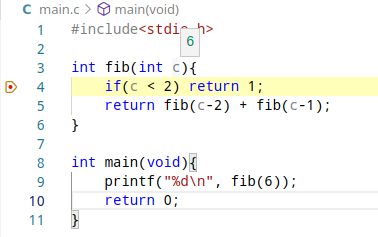
\includegraphics[width=0.8\textwidth]{vscode-dbg-decoration.png}
    \caption[]{Esempio di decorazione del codice durante il debug.}\label{fig:vscode-dbg-dec}
\end{figure}

\section{GDB Server e Livello fisico}

Il secondo livello è costituito dal firmware presente sull'ATMega16U2 collocato sulla scheda \textit{Arduino Uno R3} (componente \texttt{U3}).

Questo firmware, completamente ripensato rispetto all'originale, si occupa di convertire i comandi inviati dall'\textit{host} tramite una connessione USB simulando un dispositivo seriale e di adattarli al \textit{debugging} tramite DebugWire, implementando un server GDB direttamente all'interno dell'integrato.

Il secondo livello si occuperà di mantenere una connessione avente stato con il \textit{debugger}, ``tradurre'' i comandi GDB in modo che possano essere inoltrati al target tramite protocollo DebugWire e garantire funzionalità aggiuntive quali un livello di comunicazione \textit{target-to-host} su connessione di debug nominato Real Time Terminal (RTT).

Il firmware dell'ATMega16U2 è composto da quattro macro componenti logiche descritte a seguire in questa relazione:
\begin{enumerate}
    \item Comunicazione USB con l'\textit{host}, implementata grazie all'utilizzo di una libreria esterna (LUFA\footnote{https://github.com/abcminiuser/lufa}).
    \item Server GDB
    \item Implementazione dell'interfaccia seriale open collector
    \item Implementazione del protocollo DebugWire
\end{enumerate}

\subsection{Protocollo GDB}

Il protocollo per la comunicazione client-server di GDB è definito a partire da un canale di comunicazione in grado di trasmettere caratteri \textit{ASCII}.
Così facendo è possibile trasmettere anche su canali strettamente testuali e non standard (simboli da 7 bit).

Affinché sia possibile trasmettere dati in tale formato è necessario ricorrere alla codifica esadecimale testuale dei numeri come definita dai \cref{lst:nib-2-char,lst:char-2-nib} i quali rappresentano due funzioni di conversione da intero a esadecimale testuale e viceversa.
Si noti come nelle funzioni si parli di \textit{nibble}, ovvero un'unità di quattro bit (che possono prendere valori compresi tra 0 e 15). Questo perché un byte viene convertito in due caratteri alfabetici per essere rappresentato in esadecimale e, similmente, due caratteri alfabetici rappresentano un solo byte.

\noindent\begin{minipage}{\textwidth}
    \begin{lstlisting}[style=C, caption={Funzione di conversione da nibble a carattere alfabetico}, label=lst:nib-2-char]
    char nib2hex(unsigned char nib){
        /*
            Se il valore da mappare è minore di dieci allora sarà una cifra
        */
        if(nib < 10) return nib + '0'; 

        /*
            Altrimenti sarà una lettera (minuscola)
        */
        return nib - 10 + 'a';
    }
    \end{lstlisting}
\end{minipage}

\noindent\begin{minipage}{\textwidth}
    \begin{lstlisting}[style=C, caption={Funzione di conversione da carattere alfabetico a nibble}, label=lst:char-2-nib]
    unsigned char hex2nib(char hex){
        /*
            Se il valore è una cifra allora ricaviamo l'offset dalla cifra `0' in quanto sequenziali
        */
        if(hex >= '0' && hex <= '9') return hex - '0';
        /*
            Altrimenti riproponiamo per la lettera 'a' + 10
        */
        return hex - 'a' + 10;
    }
    \end{lstlisting}
\end{minipage}

I valori stabiliti negli offset sono di facile interpretazione: si ricordi che nel linguaggio C i caratteri hanno lo stesso significato di interi a otto bit, di conseguenza è possibile sommare o sottrarre caratteri i quali verranno interpretati con il loro relativo valore numerico assegnato dalla tabella \textit{ASCII}. 

In particolare il carattere `a' corrisponde al valore esadecimale 0x41 e il carattere `0' corrisponde al valore 0x30. Si ricordi che le cifre numeriche e le lettere, siano esse minuscole o minuscole, sono sequenziali in tale tabella.

Il protocollo GDB, inoltre, permette al server --- quando il target non è in stato di \textit{halt} --- di inviare notifiche da mostrare a schermo mediante il comando `\texttt{O}'.

Questa funzionalità sarà la base per l'implementazione del terminale in tempo reale.

\subsubsection{Formato}

I pacchetti inviati sul canale di comunicazione, come mostrato dalla \cref{fig:gdb-packet}, sono composti da una sezione contenente il comando e delimitata dai caratteri \texttt{\$} e \texttt{\#} seguita da due caratteri esadecimali rappresentanti un byte di controllo il cui valore è dato dall'\cref{eq:gdb-checksum}

\begin{figure}[t]
    \centering
    \begin{bytefield}[endianness=big,bitwidth=1em]{32}
        \bitbox{4}{\$} & \bitbox{20}{cmd} & \bitbox{4}{\#} & \bitbox{4}{CHKSM}\\
    \end{bytefield}
    \caption[]{Struttura di un pacchetto utilizzato nella comunicazione client-server GDB.}\label{fig:gdb-packet}
\end{figure}

\begin{equation}\label{eq:gdb-checksum}
    CHKSM = byte2asciihex \left( \left(\sum_{1=0}^{\# cmd} cmd_i\right) \ \bmod{256}\right)
\end{equation}

Questa procedura permette di implementare un parser di comandi a bassissimo impatto sulla memoria SRAM in quanto è possibile calcolare il \textit{checksum} durante la ricezione.

Il formato dei comandi è generalmente definito come una lettera alfabetica seguita da una serie di parametri separati dal carattere virgola e a seguire gli argomenti, codificati in esadecimale alfabetico, separati dai parametri tramite i due punti\cite{site:gdbproto}.